%!TEX root=../thesis.tex
\chapter{The PROSIT tool}\label{chp:tool}

% + LA BASE DA CUI PARTIRE E' IL PAPER \ref{prosit}
% + struttura dei moduli principali + linguaggio + librerie utilizzate + OOP patterns 
% + use cases diagram (vedi paper) 
% + focus nella creazione dei task RR (qbd_rr_colver.cpp) e di come abbiamo migliorato
%   la creazione della matrice (costruita in 3 fasi separate) in modo da sfruttare a pieno
%   le regolarità presenti al suo interno --> dati su quanto siano migliorate le performance 
%   dopo le modifiche (vedi mail con Bernardo per i numeri)
% + approssimazione conservativa della PMF (sia in alto che in basso)
% + distinzione solver da linea di comando e per xml
%     [+] solver_command_line e descrizione parametri in input
%     [+] xml_solver con esempi di chiamata + spiegazione struttura dell'xml da dare in input
% + descrizione web interface e motivi per cui è stata fatta (facilità d'uso per la creazione
%   dell'xml da zero)

PROSIT is a tool that facilitates the access to probabilistic analysis in the area of soft real-time systems. For resource reservation task, the tool offers a quality metric related to the probabilistic behaviour of the task. The fixed priority type of task is currently under development and it is not available yet.\\
Moreover it also gives the possibility to execute an automatic procedure for the \emph{synthesis} of scheduling parameters that optimise a certain QoS.

\section{Internal structure}\label{structure}
PROSIT is written in C++ and it has a modular structure, as the Object Oriented Programming (OOP) paradigm implicitly suggests.\\
Some external libraries are used in order to increase the performance during the matrices/vectors operarions and to simplify the data structure management. The most relevant are \emph{Eigen}\footnote{\url{http://eigen.tuxfamily.org}}, \emph{TinyXML-2}\footnote{\url{https://github.com/leethomason/tinyxml2}} and \emph{Doxygen}\footnote{\url{http://www.stack.nl/~dimitri/doxygen/}}.
\begin{itemize}
  \item Eigen is the most important library for the tool's core, since performance can become a real problem when the matrices have several hundreds of rows and columns. It is versatile, it supports matrices and vectors of all sizes (both fixed and dynamic), it offers many primitives to modify the supported data structures, it is reliable and very fast.
  \item TinyXML-2 is used in the parser for the XML files used as input for the solver. It provides APIs to access the XML inner structure (which is treated as a Document Object Model) as C++ objects that can be easily browsed and manipulated.
  \item Doxygen is a documentation generator for multiple programming languages. It is widely used because it is highly configurable, it can extract the codebase structure (like class diagrams and many others) even from undocumented files and especially because it is possible to select the output format for the documentation (such as HTML, {\LaTeX} and Unix man pages).
\end{itemize}

Figure \ref{classdiagram} displays an overview of the internal structure of PROSIT, presented in the form of a class diagram. This image can be useful to better understand the tool's modular structure. PROSIT can be divided into a few of standalone modules:
\begin{itemize}
  \item the distribution handler class for both PMFs and CDFs.
  \item the task descriptor class, where the inner structure of a task is described and stored.
  \item the XML parser and the utilities for the XML manipulation.
  \item the probability solver class that is essentially a wrapper object for the solving algorithms and the parameters for the RR task.
  \item the QBDP interpretation for the input task; this class actually implements the functions to build the transition matrix and the solution algorithm for the probability solver.
  \item the QoS function; it is used to compute the final value for the Quality of Service given the input task parameters.
  \item the command line and the XML solvers contains the \emph{main} function that are compiled in order to obtain the executable files.
\end{itemize}   

\begin{figure}[H]
  \center{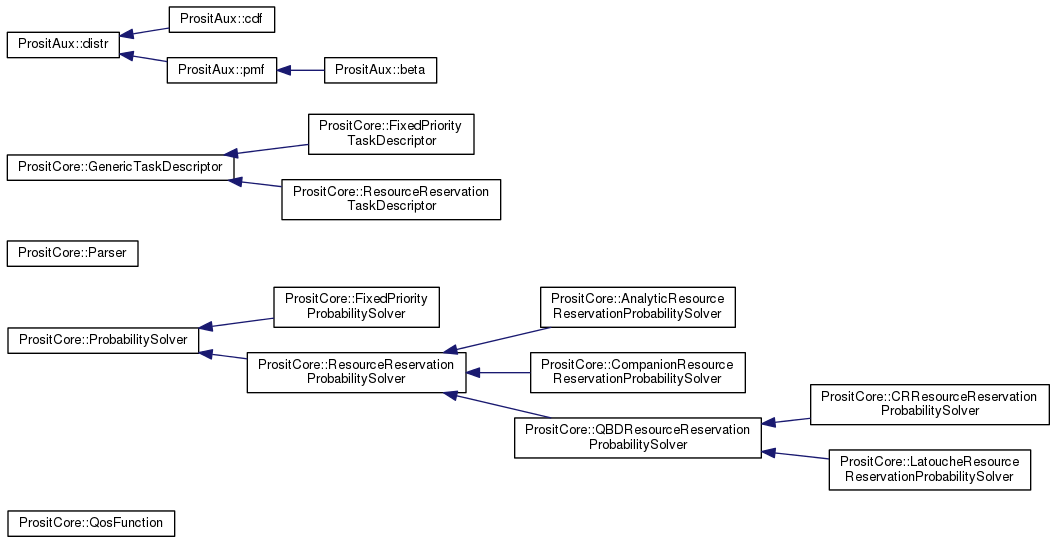
\includegraphics[width=0.85\linewidth]{classdiagram.png}}
  \caption{The class diagram generated by Doxygen.}
  \label{classdiagram}
\end{figure}

\section{Use cases}
The most common use case for PROSIT is the \emph{analysis problem}: the users are required to enter the parameters to define the task/s to be analysed.\\
Since a task can only be of resource reservation type, the values for the time requirements (namely the PMF for the computation time and the one for the inter-arrival time, which is essential if the task is aperiodic) and the scheduling parameters (\( Q_{i}^s \) and \( T_{i}^s \)) need to be provided. Thanks to the temporal isolation property defined in Equation \ref{schedCond}, if several tasks are specified as input, the tool is allowed to treat every task as if it executes on a different CPU. It is possible to easily understand that this situation leads to additional simplifications during the design phase.\\ 
The distribution functions can be specified either inside the task section in the XML file or retrieved from a text file.
\begin{figure}[H]
  \center{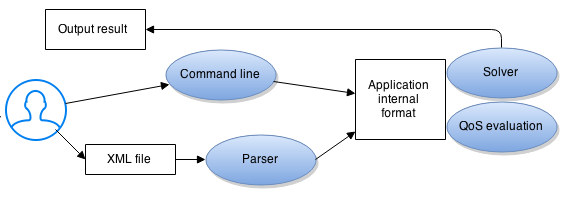
\includegraphics[width=0.57\linewidth]{usecase.png}}
  \caption{The analysis use case.}
  \label{usecase}
\end{figure}

As a result of an invocation of the tool, all the information provided by the user are analysed and then the solver for the probabilistic deadlines is called.\\ 
The \emph{apply\_algorithm()} method called by the probability solver object is a pure virtual function\footnote{Pure virtual functions in C++ are used to take advantage of polymorphism. This is essential for providing a unique interface for multiple derived objects implementing different versions of the same method. See Figure \ref{classdiagram}.}. This choice allows PROSIT to call the right solution strategy selected by the user.\\
The final results and their computation times are either printed on the screen or written on a text file.

\section{RR solver}
The solver for resource reservation tasks is based on algorithms for a numerical solution of the connected Quasi-Birth-Death process. It implements the following methods:
\begin{lstlisting}[frame=bt]
  void pre_process();
  bool compute_pi0();
  void post_process();
  void fill_in_probability_map();
\end{lstlisting}

The \emph{pre\_process()} function creates the matrices used by the QBD algorithms, which are implemented in every derived class under the name of \emph{apply\_algorithm()}. The second method is responsible for computing the probabilities from the matrix mentioned in the previous step. \emph{Post\_process()} guarantees that the algorithm gives a reasonable output, while the method \emph{fill\_in\_probability\_map()} fills the map used to store the computation results.\\
The solver invokes these functions in the order they were presented.

\subsection{Conservative approximation for PMF}
The approximation described in this section is performed to obtain a compromise between accuracy and computation time. Since the size of the transition matrix is directly proportional to the one of the PMF, reducing the size of the PMF will lead to a smaller matrix and a faster computation.\\  
In order to obtain a \emph{conservative approximation}, the values of the PMFs for both computation and inter-arrival times need to be \emph{resampled} to an integer value\footnote{In the probabilistic deadline \emph{(t,\,p)}, both the time and the probability values can be expressed as floating point numbers. Internally, PROSIT approximates the time values to an integer since we aim to output an estimate.} before building the transition matrix.\\
The way of reasoning is the same for both cases, but with a very important detail: a computation time has to be approximated to a greater value, while an inter-arrival time has to be rounded to a lower one. In this way a task arrives slightly earlier and executes for a longer period of time.\\ 
This procedure is necessary because the tool must always be placed into a \emph{worst-case scenario}. The resampling function returns a pointer to the resampled PMF object and it is defined as follows:
\begin{lstlisting}[frame=bt, numbers=none]
  pmf * resample(int granularity, bool direction);
\end{lstlisting}

where \emph{granularity} is the desired width for the bins of the resampled PMF and \emph{direction} is a flag used to make the approximation either to a grater or a lower value, depending on the type of the calling object. An example of a resampled normal distribution is illustrated in Figure \ref{resample}.\\
\begin{figure}[H]
  \center{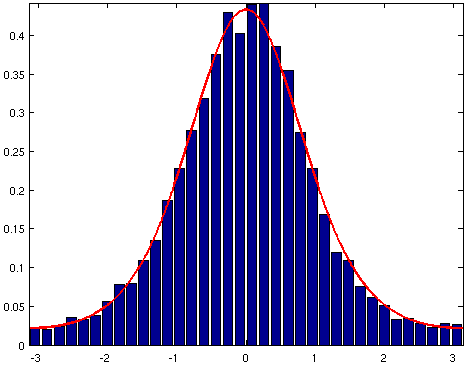
\includegraphics[width=0.4\linewidth]{resample.png}}
  \caption{A normal distribution (red) resampled at 36 bins (blue).}
  \label{resample}
\end{figure}

\subsection{Transition matrix creation} \label{matrixcreation}
In order to create the transition matrix it is possible to proceed with two different approaches: one is to fill the matrix cell by cell, while the other is to exploit its internal structure described also in Section \ref{mcconcepts}.
\begin{equation*}
  P = 
  \begin{bmatrix}
    C & A_{0} & 0 & 0 & 0 & \cdots \\
    A_{2} & A_{1} & \ddots & 0 & 0 & \cdots \\
    0 & \ddots & \ddots & A_{0} & 0 & \cdots \\
    0 & 0 & A_{2} & A_{1} & \ddots & \cdots \\
    \cdots & \cdots & \cdots & \ddots & \ddots & \ddots
  \end{bmatrix}
\end{equation*}

The creation of the transition matrix used as input for the solution algorithms can result in a critical performance bottleneck, since the size can be huge\footnote{Some tests were performed with a matrix size of 100 up to nearly one thousand.}.\\ 
Given that the complexity and the overall performance of the algorithms mentioned in Section \ref{benefits} cannot be changed\footnote{The arithmetic complexity of the Cyclic Reduction algorithm is \( O(n\log_2n) \), for the Latouche-Ramaswami it is \( O(n^{2}) \) and the one for the Companion is also quadratic.}, this will certainly explain the motivation behind the effort to optimize as much as possible the matrix creation phase.\\
As explained in Section \ref{transitionmatrix}, the whole transition matrix has a recurrent block structure. The first step is to limit the matrix size to the one of \( C \), \( A_{0} \), \( A_{1} \) and \( A_{2} \), since the matrix can theoretically have an infinite size that makes it intractable computationally speaking. First of all the \( max_{rows} \) and \( max_{cols} \) values need to be computed. They represent the maximum possible number of rows and columns respectively and they can be evaluated as follows: 
\begin{equation*}
\begin{split}
  max_{rows} &= i.get\_min() * Q + 1 \\
  max_{cols} &= c.get\_max() - c.get\_min() + 1
\end{split}
\end{equation*}

where \( i.get\_min() \) returns the minimum value for the inter-arrival time PMF, \( c.get\_max() \) returns the maximum value for the computation time PMF, \( c.get\_min() \) returns the minimum value for the computation time PMF and \( Q \) is the budget associated with the given task.\\
After taking \( max_{v} = max\,\{max_{rows}\,,\,max_{cols}\} \) as the size of one of the above mentioned submatrices, it is possible to know that the required size of the whole transition matrix \( P \) is equal to \( 2 \times max_{v} \).\\
The approach used to calculate the values inside the matrix is based on its internal structure, which is proven in \cite{pipelines} to be like:
\begin{figure}[H] \label{matrixstructure}
\begin{equation*} 
  P_{i} = 
  \begin{bmatrix}
    a_{i,0} & a_{i,1} & a_{i,H_{i}} & 0 & 0 & 0 & 0 & 0 & 0 & 0 \\
    \vdots & \vdots & \vdots & \vdots & \vdots & \vdots & \vdots & \vdots & \vdots & \vdots\\
    a_{i,0} & a_{i,1} & a_{i,H_{i}} & 0 & \cdots & \cdots & \cdots & \cdots & \cdots & \cdots \\
    b_{i,0,0} & b_{i,0,1} & b_{i,0,H_{i}} & b_{i,0,H_{i}+1} & 0 & \cdots & \cdots & \cdots & \cdots & \cdots \\
    b_{i,0,0} & b_{i,0,1} & b_{i,0,H_{i}} & b_{i,0,H_{i}+1} & b_{i,0,H_{i}+2} & 0 & \cdots & \cdots & \cdots & \cdots \\
    \vdots & \vdots & \vdots & \vdots & \vdots & \vdots & \ddots & \vdots & \vdots & \vdots \\
    b_{i,G_{i},0} & b_{i,G_{i},1} & \cdots & b_{i,G_{i},H_{i}} & b_{i,G_{i},H_{i}+1} & \cdots & \cdots & b_{i,G_{i},F_{i}} & 0 & \cdots \\
    0 & c_{i,0} & c_{i,1} & \cdots & c_{i,H_{i}} & c_{i,H_{i}+1} & \cdots & c_{i,F_{i}-1} & c_{i,F_{i}} & \ddots \\
    \vdots & \ddots & \ddots & \ddots & \ddots & \ddots & \ddots & \ddots & \ddots & \ddots
  \end{bmatrix}
\end{equation*}
\caption{The transition matrix for the generic \( i^{th} \) stage.}
\end{figure}

The matrix shown above describes the \( P_{i} \) matrix where it is possible to spot an internal recurrent configuration that is highlighted with the different names for the rows (\emph{a}, \emph{b} and \emph{c}).\\
To take advantage of this proprerty, the \emph{pre\_process()} method builds the matrix in \textbf{three steps}: the first one is to calculate only the first row and then copy its values until the end of the \emph{"a"} block. Secondly all the \emph{transient} rows denoted with the letter \emph{"b"} are calculated cell by cell. This part of the matrix exists only if the task is aperiodic. In the case of a periodic one the transition matrix is composed only by the blocks named with \emph{a} and \emph{c}. The algorithm is written to fit both the cases, but if an aperiodic task is given as input the transient rows are skipped.\\
In the \emph{"c"} block only the first row is calculated and then it is copied to the following one shifted right by one and padding with zero the leftmost element.\\
Exploiting as much as possible the internal structure of the matrix \( P_{i} \) prevents the algorithm from calculating every single cell of the matrix, which involves a function to be called \( max_{v}^{2} \) times. The time needed to calculate the entire matrix with the new method decreased of around 40\% even though the overall complexity is still an \( O(n^{2}) \). For more details about this result see Section \ref{matrixperformance}.

\section{Tool's execution}
As presented in Section \ref{structure}, the compilation process generates two executable files that can run from a terminal shell: the \emph{command line} and the \emph{XML} solver. They provide two slightly different interfaces for the tool and they are described in detail in this section. Every parameter describing a time value is measured in microseconds.

\subsection{Command line solver}
An example of shell execution for the command line solver is now provided and explained:
\begin{lstlisting}[frame=bt, numbers=none]
  ./solver <comp_time_pmf> <inter_time_pmf> [options]
\end{lstlisting}    

The parameters accepted by the \textbf{command line} solver, both in short and long form, are the following:
\begin{itemize}
  \item \texttt{comp\_time\_pmf}: is the path to the file containing the PMF of the computation time.
  \item \texttt{inter\_time\_pmf}: is the path to the file containing the PMF of the inter-arrival time.
  \item \texttt{-t (-{}-period}): sets the reservation period; it is a required argument.
  \item \texttt{-q (-{}-budget)}: sets the budget; it is a required argument and the default value is 10000.
  \item \texttt{-e (-{}-epsilon)}: sets the epsilon value used as threshold for the approximation error; the default value is \( 1 \times 10^{-14} \).
  \item \texttt{-i (-{}-max\_iterations)}: sets the maximum number of iterations for the algorithm.
  \item \texttt{-T (-{}-task\_period)}: sets the task period.
  \item \texttt{-s (-{}-step)}: sets the step for the resampling function.
  \item \texttt{-M (-{}-max\_deadline)}: sets the maximum value for the deadline.
  \item \texttt{-v (-{}-verbose)}: sets the verbose flag; it ensures that the output will provide more information to the user during the execution of the tool.
  \item \texttt{-l (-{}-latouche)}, \texttt{-c (-{}-cyclic)}, \texttt{-o (-{}-companion)}, \texttt{-a (-{}-analytic)}: set a flag used to specify the solution algorithm. 
  \item \texttt{-h (--help)}: shows all the possible parameters.
\end{itemize}
 
\subsection{XML solver}
An example of shell execution for the XML solver is now provided and explained:
\begin{lstlisting}[frame=bt, numbers=none]
  ./xml_solver <xml_file> [options]
\end{lstlisting}

The parameters accepted by the xml solver, both in short and long form, are the following:
\begin{itemize}
  \item \texttt{xml\_file}: is the path to the xml file used to define the task/s.
  \item \texttt{-v (--verbose)}: sets the verbose mode, as happens in the command line; it overrides the flag specified in the XML file.
  \item \texttt{-s (--silent)}: sets the silent mode; it overrides the flag specified in the XML file.
  \item \texttt{-h (--help)}: shows all the possible parameters.
\end{itemize}

The structure for the input file is designed in order to make the task definition easier for the user and, at the same time, more self-explanatory than a list of parameters. An example of an input file that defines a single task is shown in Figure 3.5.\\
To define multiple tasks into a single configuration file the user can simply utilize several \emph{"task"} tags inside the global \emph{"solve"} tag.\\ 
For further details about the possible values the attributes can take see the tool's documentation.  
\begin{figure}[H]
\begin{lstlisting}[frame=bt, language=XML, numbers=none]
  <solve>
    <task type="periodic" schedule="RR" name="0.3" algorithm="cyclic">
      <period>100000</period>
      <serverPeriod>25000</serverPeriod>
      <serverBudget>7500</serverBudget>
      <pmfComputation type="beta">
        <step>100</step>
        <file>test_case_1.txt</file>
      </pmfComputation>
      <pmfInterarrival type="beta">
        <step>100</step>
        <file>z_2.txt</file>
      </pmfInterarrival>
      <qosfun type="linear">
        <pmin>0.01</pmin>
        <pmax>0.95</pmax>
        <scale>0.5</scale>
        <offset>0.95</offset>
      </qosfun>
      <Delta>7500</Delta>
      <maxDeadline>4</maxDeadline>
    </task>
  </solve>
\end{lstlisting}
\caption{An example of the input XML file structure.}
\end{figure}

\section{Web interface}
The \emph{web interface} is developed in order to be as user-friendly as possible. It is designed to run on a remote server which takes care of executing an instance of the XML solver. Moreover it requires PHP and a web-server\footnote{Apache is fine, but any other web-server can manage it.} to be installed on it.\\
The \textbf{client-server} paradigm allows to move the heavy processing part from a normal laptop to a machine with more computational and memory resources. This is very useful to test the tool with many different inputs, since their execution may take several hours\footnote{The time PROSIT takes to complete its work mainly depends on the size of the transition matrix. This value is highly influenced by the granularity parameter and the reservation period \( T_{i}^{s} \) used to resample the PMF of the computation time and of the inter-arrival time. The lower the granularity is, the bigger is the transition matrix describing the relative QBDP.}.
\begin{figure}[H]
  \center{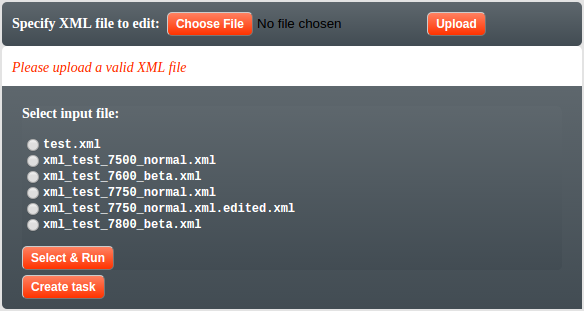
\includegraphics[width=0.7\linewidth]{index.png}}
  \caption{The homepage.}
  \label{index}
\end{figure}

Figure \ref{index} shows the homepage: it allows the user to upload XML files from his/her computer. When some input is availabe on the server it is shown in the list positioned in the middle of the page. Once a file is selected, the \emph{"select and run"} button can be clicked to start the computation phase. The output is displayed in real time.\\
Another key feature of this Graphical User Interface (GUI) is the possibility to create a task and define its parameters from scratch by clicking the \emph{"create task"} button.

\begin{figure}[H]
  \center{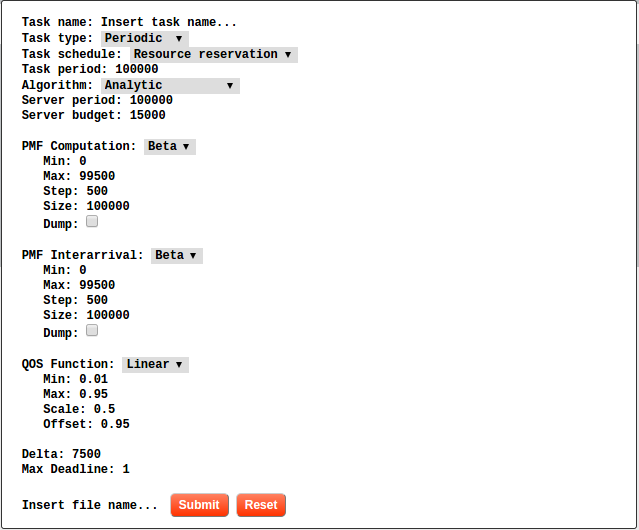
\includegraphics[width=0.7\linewidth]{modal.png}}
  \caption{The XML creator.}
  \label{modal}
\end{figure}  

As it can be seen in Figure \ref{modal}, a modal window appears on the screen. It allows the user to easily enter all the parameters to customize the task\footnote{All the fields have a default value that can be changed at will. The dropdown lists on some of the fields are thought to limit the possible choices only to the ones currently available for the tool.}; then he/she can save the selected configuration to an XML file directly on the server with the desired name. This interface makes the task creation phase a lot easier, especially for non-expert users.\\
Another feature is a live XML editing from an uploaded file (Figure \ref{editor}). This may be useful when the user would like to slightly modify some parameters for a task, without the need to edit the file locally and then upload it again on the remote machine.

\begin{figure}[H]
  \center{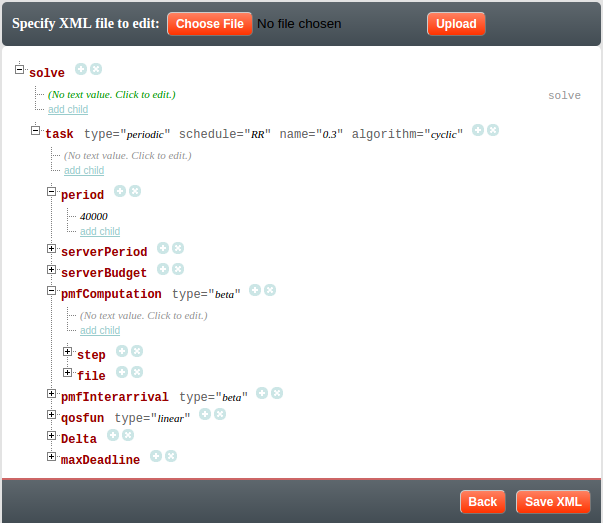
\includegraphics[width=0.7\linewidth]{editor.png}}
  \caption{The XML editor.}
  \label{editor}
\end{figure}  